\documentclass[journal,12pt,twocolumn]{IEEEtran}

\usepackage{setspace}
\usepackage{gensymb}

\singlespacing


\usepackage[cmex10]{amsmath}

\usepackage{amsthm}

\usepackage{mathrsfs}
\usepackage{txfonts}
\usepackage{stfloats}
\usepackage{bm}
\usepackage{cite}
\usepackage{cases}
\usepackage{subfig}

\usepackage{longtable}
\usepackage{multirow}

\usepackage{enumitem}
\usepackage{mathtools}
\usepackage{steinmetz}
\usepackage{tikz}
\usepackage{circuitikz}
\usepackage{verbatim}
\usepackage{tfrupee}
\usepackage[breaklinks=true]{hyperref}
\usepackage{graphicx}
\usepackage{tkz-euclide}
\usepackage{float}

\usetikzlibrary{calc,math}
\usepackage{listings}
    \usepackage{color}                                            %%
    \usepackage{array}                                            %%
    \usepackage{longtable}                                        %%
    \usepackage{calc}                                             %%
    \usepackage{multirow}                                         %%
    \usepackage{hhline}                                           %%
    \usepackage{ifthen}                                           %%
    \usepackage{lscape}     
\usepackage{multicol}
\usepackage{chngcntr}

\DeclareMathOperator*{\Res}{Res}

\renewcommand\thesection{\arabic{section}}
\renewcommand\thesubsection{\thesection.\arabic{subsection}}
\renewcommand\thesubsubsection{\thesubsection.\arabic{subsubsection}}

\renewcommand\thesectiondis{\arabic{section}}
\renewcommand\thesubsectiondis{\thesectiondis.\arabic{subsection}}
\renewcommand\thesubsubsectiondis{\thesubsectiondis.\arabic{subsubsection}}


\hyphenation{op-tical net-works semi-conduc-tor}
\def\inputGnumericTable{}                                 %%

\lstset{
%language=C,
frame=single, 
breaklines=true,
columns=fullflexible
}
\begin{document}
\newtheorem{theorem}{Theorem}[section]
\newtheorem{problem}{Problem}
\newtheorem{proposition}{Proposition}[section]
\newtheorem{lemma}{Lemma}[section]
\newtheorem{corollary}[theorem]{Corollary}
\newtheorem{example}{Example}[section]
\newtheorem{definition}[problem]{Definition}

\newcommand{\BEQA}{\begin{eqnarray}}
\newcommand{\EEQA}{\end{eqnarray}}
\newcommand{\define}{\stackrel{\triangle}{=}}
\bibliographystyle{IEEEtran}
\providecommand{\mbf}{\mathbf}
\providecommand{\pr}[1]{\ensuremath{\Pr\left(#1\right)}}
\providecommand{\qfunc}[1]{\ensuremath{Q\left(#1\right)}}
\providecommand{\sbrak}[1]{\ensuremath{{}\left[#1\right]}}
\providecommand{\lsbrak}[1]{\ensuremath{{}\left[#1\right.}}
\providecommand{\rsbrak}[1]{\ensuremath{{}\left.#1\right]}}
\providecommand{\brak}[1]{\ensuremath{\left(#1\right)}}
\providecommand{\lbrak}[1]{\ensuremath{\left(#1\right.}}
\providecommand{\rbrak}[1]{\ensuremath{\left.#1\right)}}
\providecommand{\cbrak}[1]{\ensuremath{\left\{#1\right\}}}
\providecommand{\lcbrak}[1]{\ensuremath{\left\{#1\right.}}
\providecommand{\rcbrak}[1]{\ensuremath{\left.#1\right\}}}
\theoremstyle{remark}
\newtheorem{rem}{Remark}
\newtheorem*{remark}{Remark}
\newcommand{\sgn}{\mathop{\mathrm{sgn}}}
\providecommand{\abs}[1]{\vert#1\vert}
\providecommand{\res}[1]{\Res\displaylimits_{#1}} 
\providecommand{\norm}[1]{\lVert#1\rVert}
%\providecommand{\norm}[1]{\lVert#1\rVert}
\providecommand{\mtx}[1]{\mathbf{#1}}
\providecommand{\mean}[1]{E[ #1 ]}
\providecommand{\fourier}{\overset{\mathcal{F}}{ \rightleftharpoons}}
%\providecommand{\hilbert}{\overset{\mathcal{H}}{ \rightleftharpoons}}
\providecommand{\ztrans}{\overset{\mathcal{Z}}{ \rightleftharpoons}}
\providecommand{\system}{\overset{\mathcal{H}}{ \longleftrightarrow}}
	%\newcommand{\solution}[2]{\textbf{Solution:}{#1}}
\newcommand{\solution}{\noindent \textbf{Solution: }}
\newcommand{\cosec}{\,\text{cosec}\,}
\providecommand{\dec}[2]{\ensuremath{\overset{#1}{\underset{#2}{\gtrless}}}}
\newcommand{\myvec}[1]{\ensuremath{\begin{pmatrix}#1\end{pmatrix}}}
\newcommand{\mydet}[1]{\ensuremath{\begin{vmatrix}#1\end{vmatrix}}}
\numberwithin{equation}{subsection}
\makeatletter
\@addtoreset{figure}{problem}
\makeatother
\let\StandardTheFigure\thefigure
\let\vec\mathbf
\renewcommand{\thefigure}{\theproblem}
\def\putbox#1#2#3{\makebox[0in][l]{\makebox[#1][l]{}\raisebox{\baselineskip}[0in][0in]{\raisebox{#2}[0in][0in]{#3}}}}
     \def\rightbox#1{\makebox[0in][r]{#1}}
     \def\centbox#1{\makebox[0in]{#1}}
     \def\topbox#1{\raisebox{-\baselineskip}[0in][0in]{#1}}
     \def\midbox#1{\raisebox{-0.5\baselineskip}[0in][0in]{#1}}
\vspace{3cm}
\title{GATE ASSIGNMENT 1}
\author{Vojeswitha Gopireddy \\ AI20BTECH11024}
\maketitle
\newpage
\bigskip
\renewcommand{\thefigure}{\theenumi}
\renewcommand{\thetable}{\theenumi}
Download all python codes from 
\begin{lstlisting}
https://github.com/V-Gopireddy/EE3900/blob/main/GATE_Assignment1/codes/GateAssignment-1.py
\end{lstlisting}
%
and latex-tikz codes from 
%
\begin{lstlisting}
https://github.com/V-Gopireddy/EE3900/blob/main/GATE_Assignment1/GateAssignment-1.tex
\end{lstlisting}
%
\section{GATE EC 2017 Q.35}
Consider the parallel combination of two LTI systems shown in the figure.

\begin{figure}[h]
    \centering
    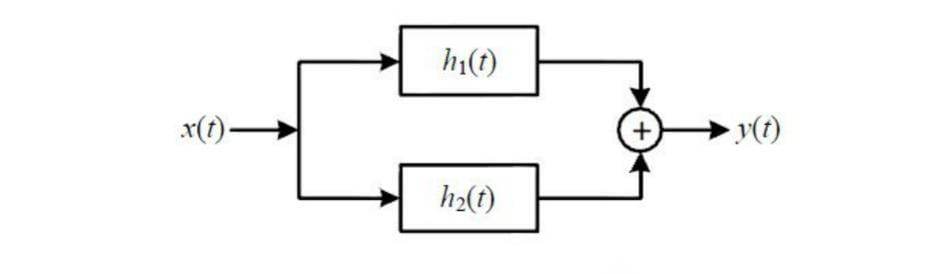
\includegraphics[width=\columnwidth]{LTI-systems.jpeg}
    %\caption{Parallel combination of two LTI systems}%
    \label{fig:my_label}
\end{figure}

The impulse responses of the systems are
\begin{align}
    h_1(t) &= 2\delta(t+2) - 3\delta(t+1)\\
    h_2(t) &= \delta(t-2)
\end{align}
If the input $x(t)$ is a unit step signal, then find the energy of $y(t)$. 
%
\section{Solution}
\begin{definition}[Laplace Transform]
It is an integral transform that converts a function of a real variable $t$ to a function of a complex variable $s$. The Laplace transform of $f(t)$ is denoted by $\mathcal{L}\cbrak{f(t)}$ or $F(s)$.
\begin{align}
    F(s)=\mathcal{L}\cbrak{f(t)}=\int_{0}^{\infty}e^{-st}f(t)dt
\end{align}
\end{definition}
\begin{definition}[Bilateral Laplace Transform]
The Laplace transform can be alternatively defined as the bilateral Laplace transform, by extending the limits of integration to be the entire real axis\\
The bilateral laplace transform of $f(t)$ is denoted by $\mathcal{L}_b\cbrak{f(t)}$ or $F_b(s)$.
\begin{align}
    F_b(s)=\mathcal{L}_b\cbrak{f(t)}=\int_{-\infty}^{\infty}e^{-st}f(t)dt
\end{align}
\end{definition}
\begin{lemma}
Linearity of bilateral laplace transform
\begin{align} 
    \mathcal{L}_b\cbrak{af(t)+bg(t)} = a\mathcal{L}_b\cbrak{f(t)}+b\mathcal{L}_b\cbrak{g(t)}\label{eq:linearity}
\end{align}
\begin{proof}
 \begin{align}
     &\mathcal{L}_b\cbrak{af(t)+bg(t)} \\&= \int_{-\infty}^{\infty}e^{-st}\cbrak{af(t)+bg(t)}dt\\
     &= a\int_{-\infty}^{\infty}e^{-st}f(t)dt+b\int_{-\infty}^{\infty}e^{-st}g(t)dt\\
     &= a\mathcal{L}_b\cbrak{f(t)}+b\mathcal{L}_b\cbrak{g(t)}
 \end{align}
\end{proof}
\end{lemma}
\begin{lemma}
For any real number c, 
\begin{align}
    \mathcal{L}_b\cbrak{u(t-c)}=\dfrac{e^{-cs}}{s}, s>0
    \label{eq:u}
\end{align}
\end{lemma}
\begin{proof}
 \begin{align}
     \mathcal{L}_b\cbrak{u(t-c)}&=\int_{-\infty}^{\infty}e^{-st}u(t-c)dt=\int_{c}^{\infty}e^{-st}dt\\
     &=\sbrak{-\dfrac{e^{-st}}{s}}_{c}^{\infty}=\dfrac{e^{-cs}}{s}, s>0
 \end{align}
\end{proof}
\begin{lemma}
For any real number c,
\begin{align}
     \mathcal{L}_b\cbrak{\delta(t-c)}=e^{-cs}, s>0\label{eq:d}
\end{align}     
\end{lemma}
\begin{proof}
 Let $f_k(t-a)$ be a function defined as,
 \begin{align}
     f_k(t-c)&= \begin{cases}
    \frac{1}{k}, & c \leq t < c+k \\~\\[-1em]
	0, & \text{otherwise}
	\end{cases}\\
	\implies\lim_{k \to 0} f_k(t-c) &= \delta(t-c)
 \end{align}
\begin{align}
     \mathcal{L}_b\cbrak{\delta(t-c)}&=\int_{-\infty}^{\infty}e^{-st}\delta(t-c)dt\\&=\lim_{k \to 0}\int_{-\infty}^{\infty}e^{-st}f_k(t-c)dt\\
     &=\lim_{k \to 0}\sbrak{-\dfrac{e^{-st}}{ks}}_{c}^{c+k}\\&= \lim_{k \to 0}\dfrac{e^{-sc}-e^{-s(c+k)}}{sk} =e^{-cs}, s>0
\end{align}     
\end{proof}
\begin{definition}[Inverse Bilateral Laplace Transform]
It is the transformation of a bilateral Laplace transform into a function of time. If $F(s)=\mathcal{L}_b\cbrak{f(t)}$, then the Inverse bilateral laplace transform of $F(s)$ is $\mathcal{L}_{b}^{-1}\cbrak{F(s)}=f(t)$.
\end{definition}
\begin{lemma}
Linearity of Inverse Bilateral Laplace Transform
\begin{align}
    \mathcal{L}_{b}^{-1}\cbrak{af(t)+bg(t)} = a\mathcal{L}_{b}^{-1}\cbrak{f(t)}+b\mathcal{L}_{b}^{-1}\cbrak{g(t)}\label{eq:linearity-1}
\end{align}
\end{lemma}
\begin{theorem}[Convolution Theorem] \label{ct}
Let $F(s)$ and $G(s)$ be the Bilateral Laplace-transform of two functions $f(t)$ and $g(t)$ respectively. Then
\begin{align}
\mathcal{L}_{b}\cbrak{f(t) * g(t)}=F(s)G(s)
\end{align}
\end{theorem}
Given that,
\begin{align}
    x(t) &= u(t)\label{eq:x}
\end{align}
And,
\begin{align}
    h_1(t) &= 2\delta(t+2) - 3\delta(t+1)\\
    h_2(t) &= \delta(t-2)
\end{align}
Since the systems are in parallel,\\
Overall impulse response of the system is,
\begin{align}
    h(t) &= h_1(t) + h_2(t)\\  &= 2\delta(t+2) - 3\delta(t+1) + \delta(t-2)
\end{align}
From \eqref{eq:d} and \eqref{eq:linearity} we have
\begin{align}
    H(s) = \mathcal{L}_{b}\cbrak{h(t)} = 2e^{2s}-3e^{s}+e^{-2s}
\end{align}
From \eqref{eq:x} and \eqref{eq:u} we have,
\begin{align}
    X(s) = \mathcal{L}_{b}\cbrak{u(t)} = \frac{1}{s}
\end{align}
The output signal $y(t)$ is given by,
\begin{align}
    y(t) &= x(t)*h(t)\\ 
    \implies \mathcal{L}_{b}\cbrak{y(t)} &= X(s)H(s)\\
    &= \frac{1}{s}\sbrak{2e^{2s}-3e^{s}+e^{-2s}}
\end{align}
Therefore we have,
\begin{align}
    y(t) &= \mathcal{L}_{b}^{-1}\cbrak{\frac{2e^{2s}}{s}-\frac{3e^{s}}{s}+\frac{e^{-2s}}{s}}\\
    &=2\mathcal{L}_{b}^{-1}\cbrak{\frac{e^{2s}}{s}}-3\mathcal{L}_{b}^{-1}\cbrak{\frac{e^{s}}{s}}\mathcal{L}_{b}^{-1}+\cbrak{\frac{e^{-2s}}{s}}\\
     &= 2u(t+2) -3u(t+1) + u(t-2) 
\end{align}
Solving we get,
\begin{align}
      y(t) &= 
     \begin{cases}
    2, & -2 \leq t < -1 \\~\\[-1em]
	-1, & -1 \leq t < 2 \\~\\[-1em]
	0, & \text{otherwise}
	\end{cases}
\end{align}
Energy of the output signal $E_y$ is given by,
\begin{align}
    E_y &= \int_{-\infty}^{\infty}\abs{y(t)}^2dt\\
    &= \int_{-2}^{-1}4dt + \int_{-1}^{2}dt\\
    &= 7
\end{align}
\begin{figure}[h!]
\centering
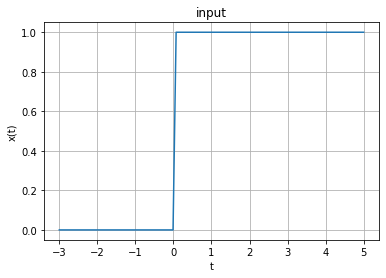
\includegraphics[width=\columnwidth]{Input-signal.png}
\caption{Input signal $x(t)$}
\label{fig:Input-signal}
\end{figure}

\begin{figure}[h!]
\centering
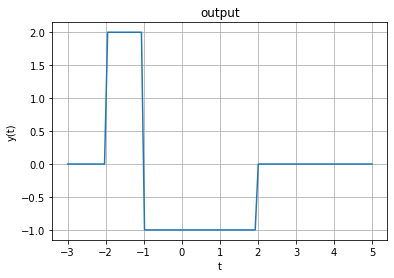
\includegraphics[width=\columnwidth]{Output-signal.png}
\caption{Output signal $y(t)$}
\label{fig:Output-signal}
\end{figure}
\end{document}